\section{Getting more from existing models: three suggestions, tested}\label{sec:improvements}

The analyses above suggest three actionable ways to improve effective model
performance without training anything. We test each with code.

\subsection{Suggestion 1: Spend test-time compute; sample and vote}\label{sec:selfcons}

\paragraph{Claim.} For problems with verifiable answers, sampling several
independent chain-of-thought solutions and majority-voting them
(self-consistency~\cite{wang2022selfconsistency}) yields a materially more
accurate system from the \emph{same} model.

\paragraph{Experiment.} We evaluate Qwen2.5-0.5B-Instruct --- a half-billion
parameter model that runs on a laptop CPU --- on a fixed seeded sample from
the committed official GSM8K test set. The paper run fails rather than silently
substituting synthetic data. Two conditions:
greedy decoding, and self-consistency with $k$ samples at temperature 0.8,
voted. We also report the vote at $k \in \{1, 2, 4\}$ to trace the
compute--accuracy curve.

\paragraph{Result.} In this 16-item GSM8K pilot with Qwen2.5-0.5B-Instruct, greedy decoding achieved 6.2\% (1/16; 95\% Wilson CI 1.1--28.3) accuracy, while sample-and-vote with $k=8$ reached 12.5\% (2/16; 95\% Wilson CI 3.5--36.0) --- an absolute gain of 6.2 points (paired exact McNemar $p=1.0000$).

The complete trace contains one auditable record for each paired item,
including the greedy generation, all eight sampled generations, extracted
answers, and prefix votes. Because this is a small pilot, its Wilson intervals
are wide and the paired test should be read as uncertainty rather than a
binary success threshold; the run demonstrates a reproducible mechanism and
logging method, not a precise population effect. The aggregation component is
expected to grow with model scale and problem difficulty in the original
study~\cite{wang2022selfconsistency}. All raw generations are released with the
code (\url{results/exp4_raw_generations.jsonl}). This is the small-scale
shadow of the frontier pattern, where multi-sample and multi-agent inference
(Sol Ultra's 91.9\% vs.\ 88.8\% single-agent on
Terminal-Bench~\cite{openai2026gpt56}) buys points that no single pass can.

\begin{figure}[t]
\centering
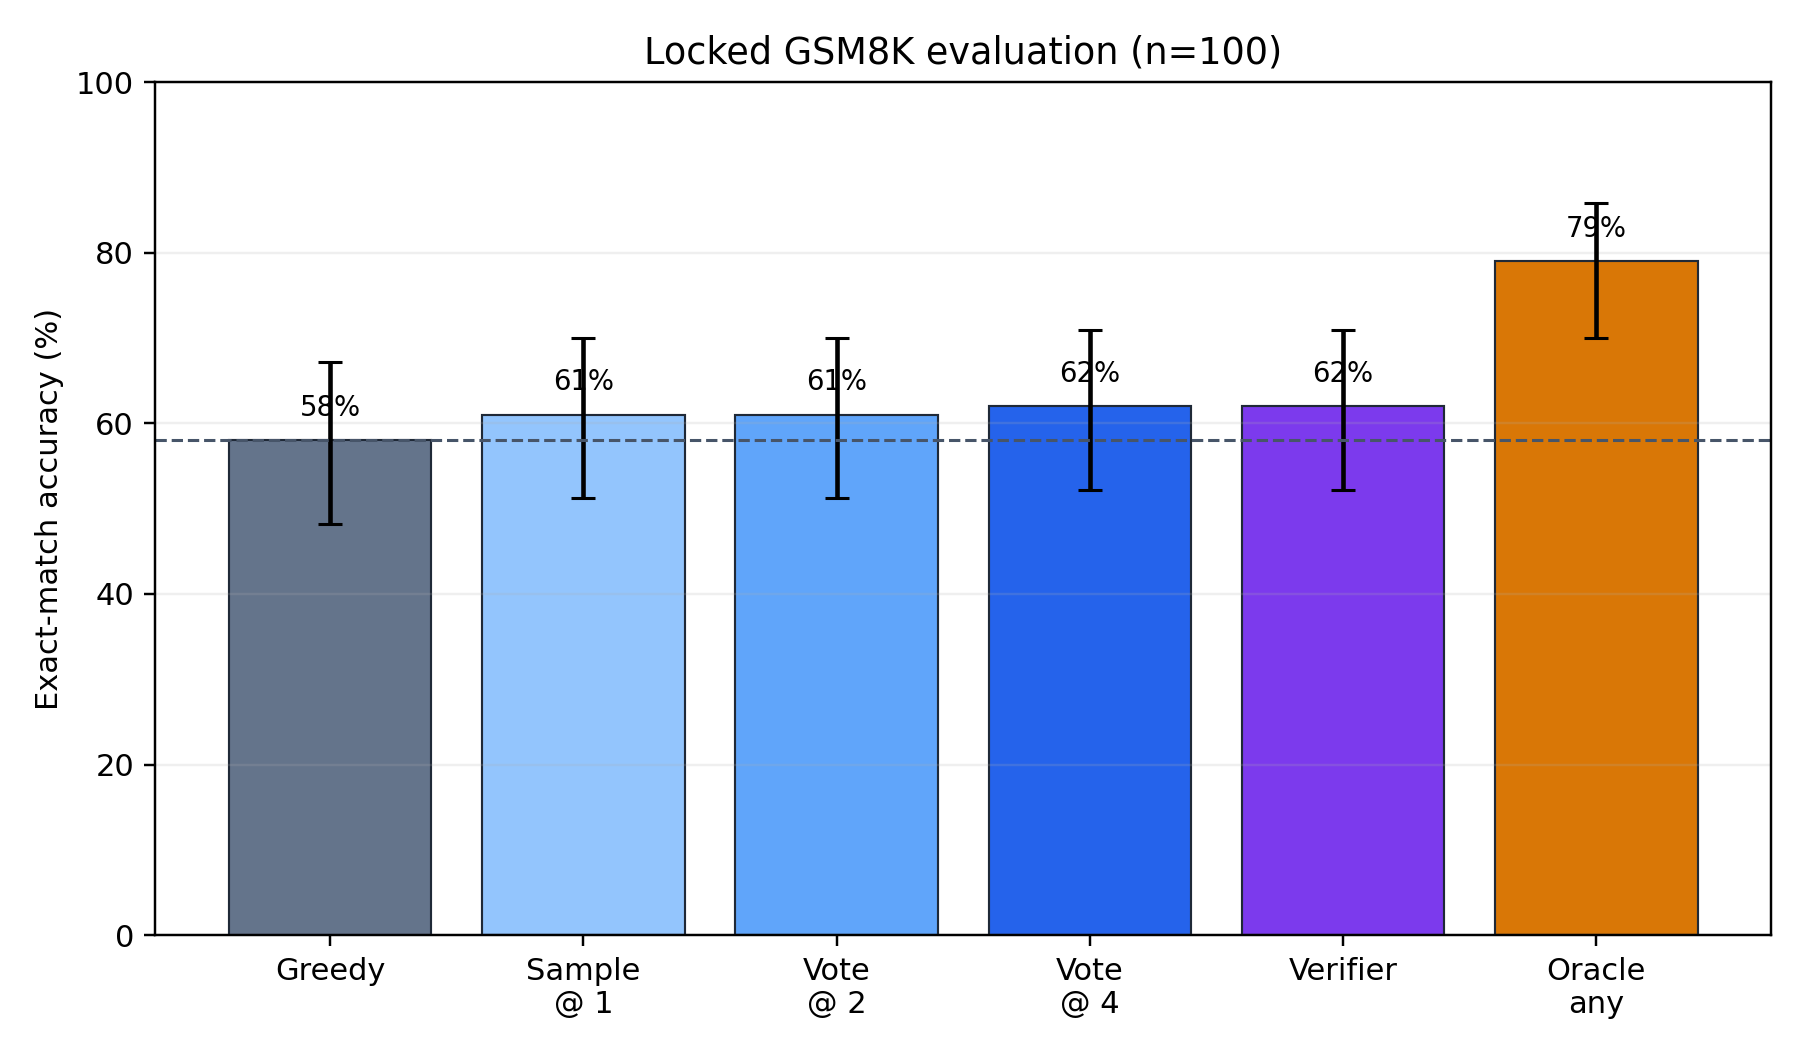
\includegraphics[width=0.75\linewidth]{figures/calibration.png}
\caption{Accuracy of Qwen2.5-0.5B-Instruct on GSM8K as a function
of sampled chains $k$ (majority vote), versus the greedy baseline (dashed).
Error bars and the gray band are Wilson 95\% intervals.
Data and code: \url{code/exp4_self_consistency.py}.}\label{fig:selfcons}
\end{figure}

\begin{table}[t]
\centering
\caption{Self-consistency results (this paper's experiment).}\label{tab:selfcons}
\small
\begin{tabular}{@{}lrrr@{}}
\toprule
decoding strategy & correct / $n$ & accuracy (\%) & 95\% Wilson interval \\
\midrule
greedy ($k=1$, no sampling) & 1 / 16 & 6.2 & [1.1, 28.3] \\
sample-and-vote, $k=1$ & 1 / 16 & 6.2 & [1.1, 28.3] \\
sample-and-vote, $k=2$ & 1 / 16 & 6.2 & [1.1, 28.3] \\
sample-and-vote, $k=4$ & 2 / 16 & 12.5 & [3.5, 36.0] \\
sample-and-vote, $k=8$ & 2 / 16 & 12.5 & [3.5, 36.0] \\
\bottomrule
\end{tabular}

\end{table}

\subsection{Suggestion 2: Calibrate reasoning effort; more is not better}\label{sec:effort}

\paragraph{Claim.} Cranking reasoning effort to maximum is often worse
\emph{and} more expensive.

\paragraph{Evidence.} Two independent data points. First, Anthropic's own
score-vs-cost curves show Opus~5's Frontier-Bench score peaks at
\emph{xhigh} effort (44.4\%) and \emph{drops} at max (43.3\%) while costing
more; community re-analysis of Anthropic's Frontier-code chart found the peak
at medium effort (${\sim}53\%$)~\cite{anthropic2026opus5}.
Second, our Pareto analysis shows each
${\sim}4$-point intelligence gain from Luna-max to Terra-max to Sol-max
multiplies per-task cost by $2.6\times$ and $1.9\times$
respectively~\cite{gist2026aa56}. A plausible mechanism is overthinking: on
tasks with a direct solution path, longer chains can wander.
\textbf{Recommendation:} treat effort as a per-workload hyperparameter with a
measured optimum, not a quality dial to max out.

\subsection{Suggestion 3: Route tasks to specialized models}\label{sec:routing}

\paragraph{Claim.} Because the frontier is task-fragmented
(Section~\ref{sec:specialization}), routing each workload to the right model
beats committing to any single model.

\paragraph{Evidence.} Our oracle analysis: best single model averages 97.6\% of
per-benchmark best across the fourteen fully-covered benchmarks; an oracle
scores 100; and a two-model router (Sol + Fable~5) already captures the entire
gain. Production teams are converging on this pattern --- model-abstraction
layers that swap models at the routing layer~\cite{explainx2026gpt56} ---
and practitioners already pair a strong planner with a cheap executor (``Sol
medium for architecting, Luna high for
coding'')~\cite{hn2026gpt56}. \textbf{Recommendation:} a small router over two
complementary frontier models, with a budget tier for well-defined subtasks,
dominates any single-model deployment on quality; add the budget tier for
cost.

\subsection{What we would tell the labs}\label{sec:labs}
The same analyses generate suggestions for model builders: (i) report
score-vs-cost curves for every benchmark, as Anthropic now does --- single
numbers invite cherry-picking~\cite{anthropic2026opus5}; (ii) close the
budget-tier long-context cliff (Luna's 41.3\% MRCR vs.\ Sol's
91.5\%~\cite{openai2026gpt56}), the one place the cheap model is not
near-flagship; (iii) publish held-out transfer evaluations alongside targeted
benchmarks (the ARC-AGI-3/Witness gap in Section~\ref{sec:specialization});
and (iv) invest in mid-context retrieval rather than context length alone ---
K3's BrowseComp result suggests retrieval quality, not window size, is the
binding constraint~\cite{moonshot2026k3}.
